\documentclass{article}
\usepackage{amsmath}
\usepackage{amsfonts}
\usepackage{amssymb}
\usepackage{amsthm}
\usepackage{geometry}
\usepackage{algorithm}
\usepackage{algpseudocode}
\usepackage{graphicx}
\usepackage{booktabs}
\usepackage{caption}
\usepackage{xcolor}
\usepackage{float}

\geometry{a4paper, left=2cm, right=2cm, top=2cm, bottom=2cm}

\title{Report for AI Capstone Homework 4:\\A Robot Manipulation Framework}
\author{FU, YONG-WEI (112550107)}
\date{\today}

\begin{document}

\maketitle

\section{Task 1: Forward Kinematics}
\subsection{Implementation of `your\_fk()` function}
The implementation of my \texttt{your\_fk()} function follows the standard 
Denavit-Hartenberg (D-H) procedure:
\begin{enumerate}
    \item \textbf{Transformation Chain:} For each joint $i \in \{1, \dots, 6\}$, a 
    $4 \times 4$ transformation matrix $A_i$ is constructed using the given D-H 
    parameters ($a_i, \alpha_i, d_i$) and the input joint angle $\theta_i$. 
    The matrix follows the D-H convention:
    \[
        A_i = \begin{bmatrix} 
            \cos\theta_i & -\sin\theta_i\cos\alpha_i & \sin\theta_i\sin\alpha_i & a_i\cos\theta_i \\
            \sin\theta_i & \cos\theta_i\cos\alpha_i & -\cos\theta_i\sin\alpha_i & a_i\sin\theta_i \\
            0 & \sin\alpha_i & \cos\alpha_i & d_i \\
            0 & 0 & 0 & 1
        \end{bmatrix}
    \]
    \begin{figure}[H]
        \centering
        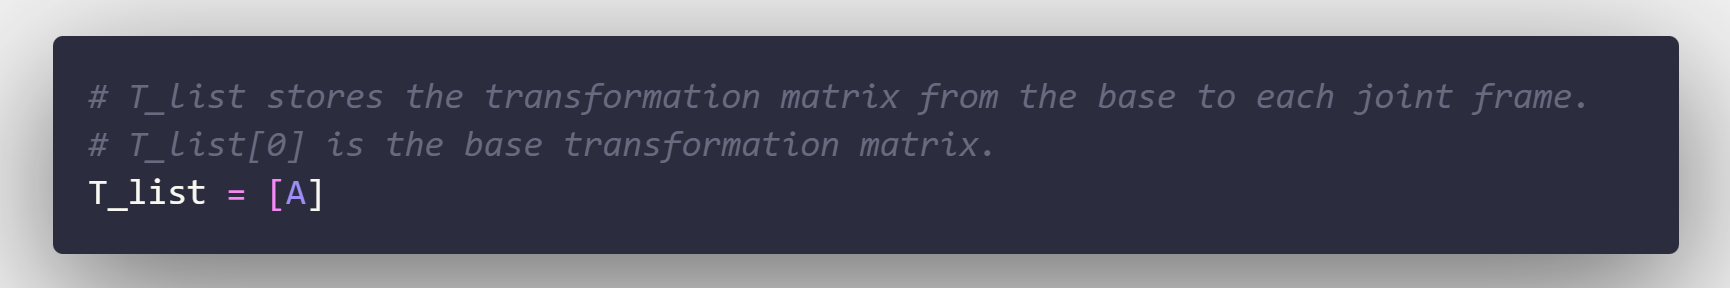
\includegraphics[width=0.8\textwidth]{screenshots/fkcode1.png}
        \caption{Code snippet for constructing the D-H transformation matrix.}
    \end{figure}

    \item \textbf{Cumulative Multiplication:} The matrices are multiplied 
    starting from the base frame transformation ($A_{base}$) to compute the 
    transformation from the world frame to the end-effector using: 
    $T = A_{base} \cdot A_1 \cdot A_2 \cdot \cdots \cdot A_6$.
    \begin{figure}[H]
        \centering
        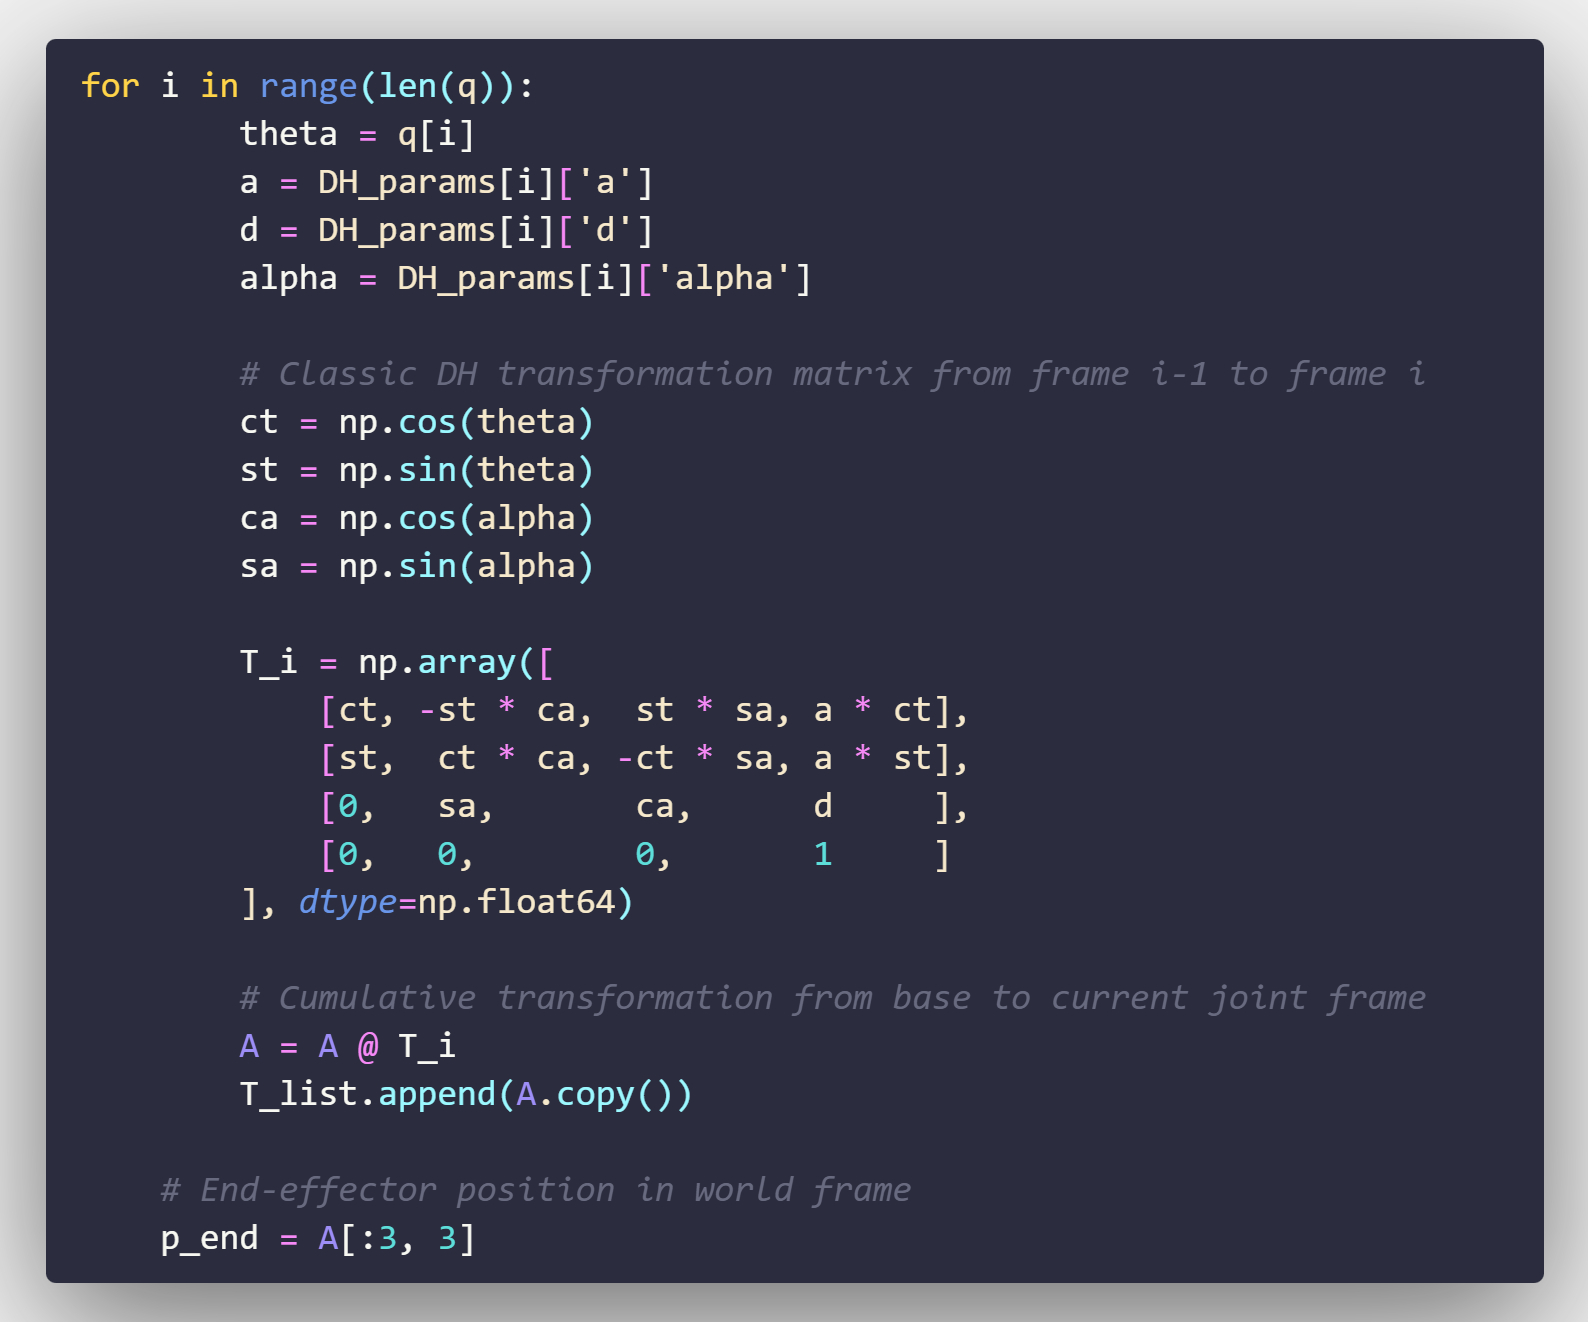
\includegraphics[width=0.8\textwidth]{screenshots/fkcode2.png}
        \caption{Code snippet for cumulative multiplication of transformation matrices.}
    \end{figure}

    \item \textbf{Geometric Jacobian Construction:} The $6 \times 6$ Jacobian matrix $J$ is built 
    column by column. For each revolute joint $i$, the $i$-th column is defined as:
    \[
        J_i = \begin{bmatrix} z_{i-1} \times (p_{end} - p_{i-1}) \\ z_{i-1} \end{bmatrix}
    \]
    where $z_{i-1}$ is the $z$-axis of frame $i-1$ and $p_{i-1}$ is its origin, both 
    expressed in the base frame.
    \begin{figure}[H]
        \centering
        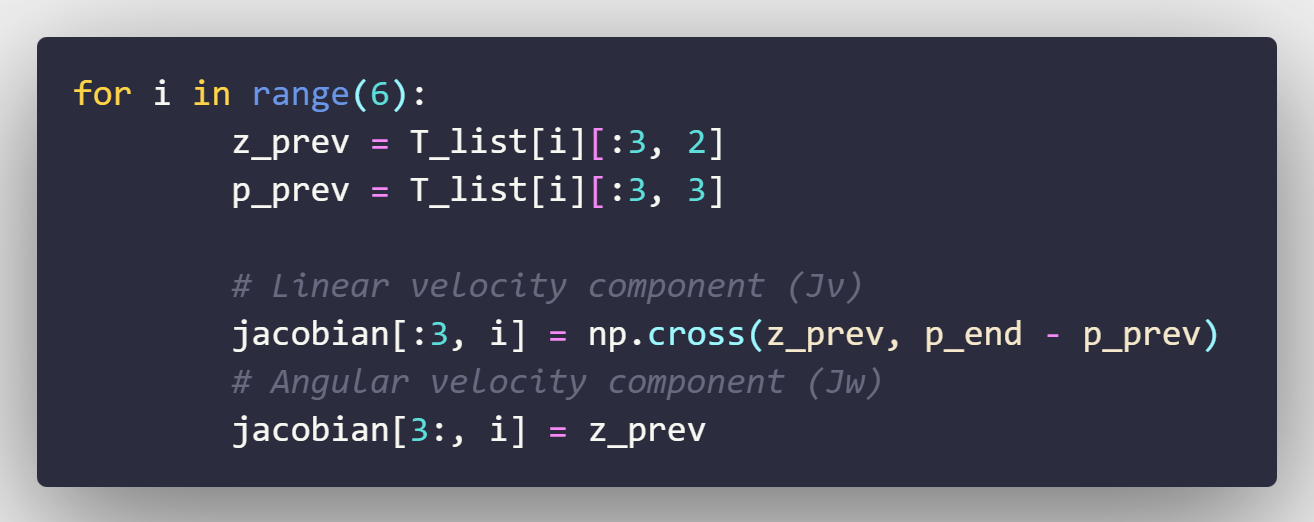
\includegraphics[width=0.8\textwidth]{screenshots/fkcode3.png}
        \caption{Code snippet for constructing the geometric Jacobian.}
    \end{figure}
\end{enumerate}

\subsection{What is the difference between D-H convention and Craig's convention (Modified D-H Convention)?}
The primary differences lie in the frame placement and the order of operations:
\begin{itemize}
    \item \textbf{Frame Assignment:} In the \textbf{Classic D-H convention}, frame $i$ is 
    attached to the end of link $i$, and the joint $i$ axis is $z_{i-1}$. In 
    \textbf{Craig's (Modified) D-H convention}, frame $i$ is attached to the beginning of link 
    $i$, and the joint $i$ axis is $z_i$.
    \item \textbf{Transformation Order:}
    \begin{itemize}
        \item \textbf{Classic:} $A_i = Rot_z(\theta_i) \cdot Trans_z(d_i) \cdot Trans_x(a_i) \cdot Rot_x(\alpha_i)$. 
        The parameters relate frame $i-1$ to frame $i$ along the common normal and the joint axis.
        \item \textbf{Modified:} $A_i = Rot_x(\alpha_{i-1}) \cdot Trans_x(a_{i-1}) \cdot Rot_z(\theta_i) \cdot Trans_z(d_i)$. 
        The parameters relate frame $i$ to frame $i-1$ (with indices shifted).
    \end{itemize}
\end{itemize}

\subsection{Complete the D-H table}
The parameters used in the implementation (based on the UR5 assignment spec) are as follows:

\begin{table}[h!]
    \centering
    \begin{tabular}{ccccc}
    \toprule
    $i$ & $d$ (m) & $\alpha$ (rad) & $a$ (m) & $\theta$ (rad) \\
    \midrule
    1 & 0.0892  & $\pi/2$  & 0      & $\theta_1$ \\
    2 & 0       & 0        & -0.425 & $\theta_2$ \\
    3 & 0       & 0        & -0.392 & $\theta_3$ \\
    4 & 0.1093  & $\pi/2$  & 0      & $\theta_4$ \\
    5 & 0.09475 & $-\pi/2$ & 0      & $\theta_5$ \\
    6 & 0.2023  & 0        & 0      & $\theta_6$ \\
    7 & 0       & 0        & 0      & 0 (Fixed) \\
    \bottomrule
    \end{tabular}
    \caption{Classic D-H parameters for the UR5 robot configuration (including fixed tool frame $i=7$).}
\end{table}

\section{Task 2: Inverse Kinematics}
\subsection{Implementation of `your\_ik()` function}
My \texttt{your\_ik()} function implements a \textbf{Numerical Inverse Kinematics} 
solver using the Jacobian Pseudo-inverse method:
\begin{enumerate}
    \item \textbf{Initialization:} The joints are initialized with a given guess \texttt{q\_init}.
    
    \item \textbf{Iteration Loop:} In each iteration (up to \texttt{max\_iters}):
    \begin{itemize}
        \item Calculate the current end-effector pose and Jacobian using \texttt{your\_fk()} I implemented earlier.
        \item \textbf{Error Calculation:} Compute the 6D error vector $\Delta x$. The position error is $p_{target} - p_{curr}$. 
        The orientation error is derived by converting the relative rotation $R_{target} \cdot R_{curr}^T$ into its axis-angle 
        representation.
        \item \textbf{Joint Update:} Compute the joint update $\Delta q = \alpha \cdot J^\dagger \cdot \Delta x$, 
        where $J^\dagger$ is the Moore-Penrose pseudo-inverse and $\alpha$ is the step size (learning rate).
        \item \textbf{Constraints:} Clip the updated joint angles $q$ within the hardware \texttt{joint\_limits}.
    \end{itemize}
    \item \textbf{Termination:} The loop stops if the norm of the 6D error falls below 
    \texttt{stop\_thresh}.

    \begin{figure}[H]
        \centering
        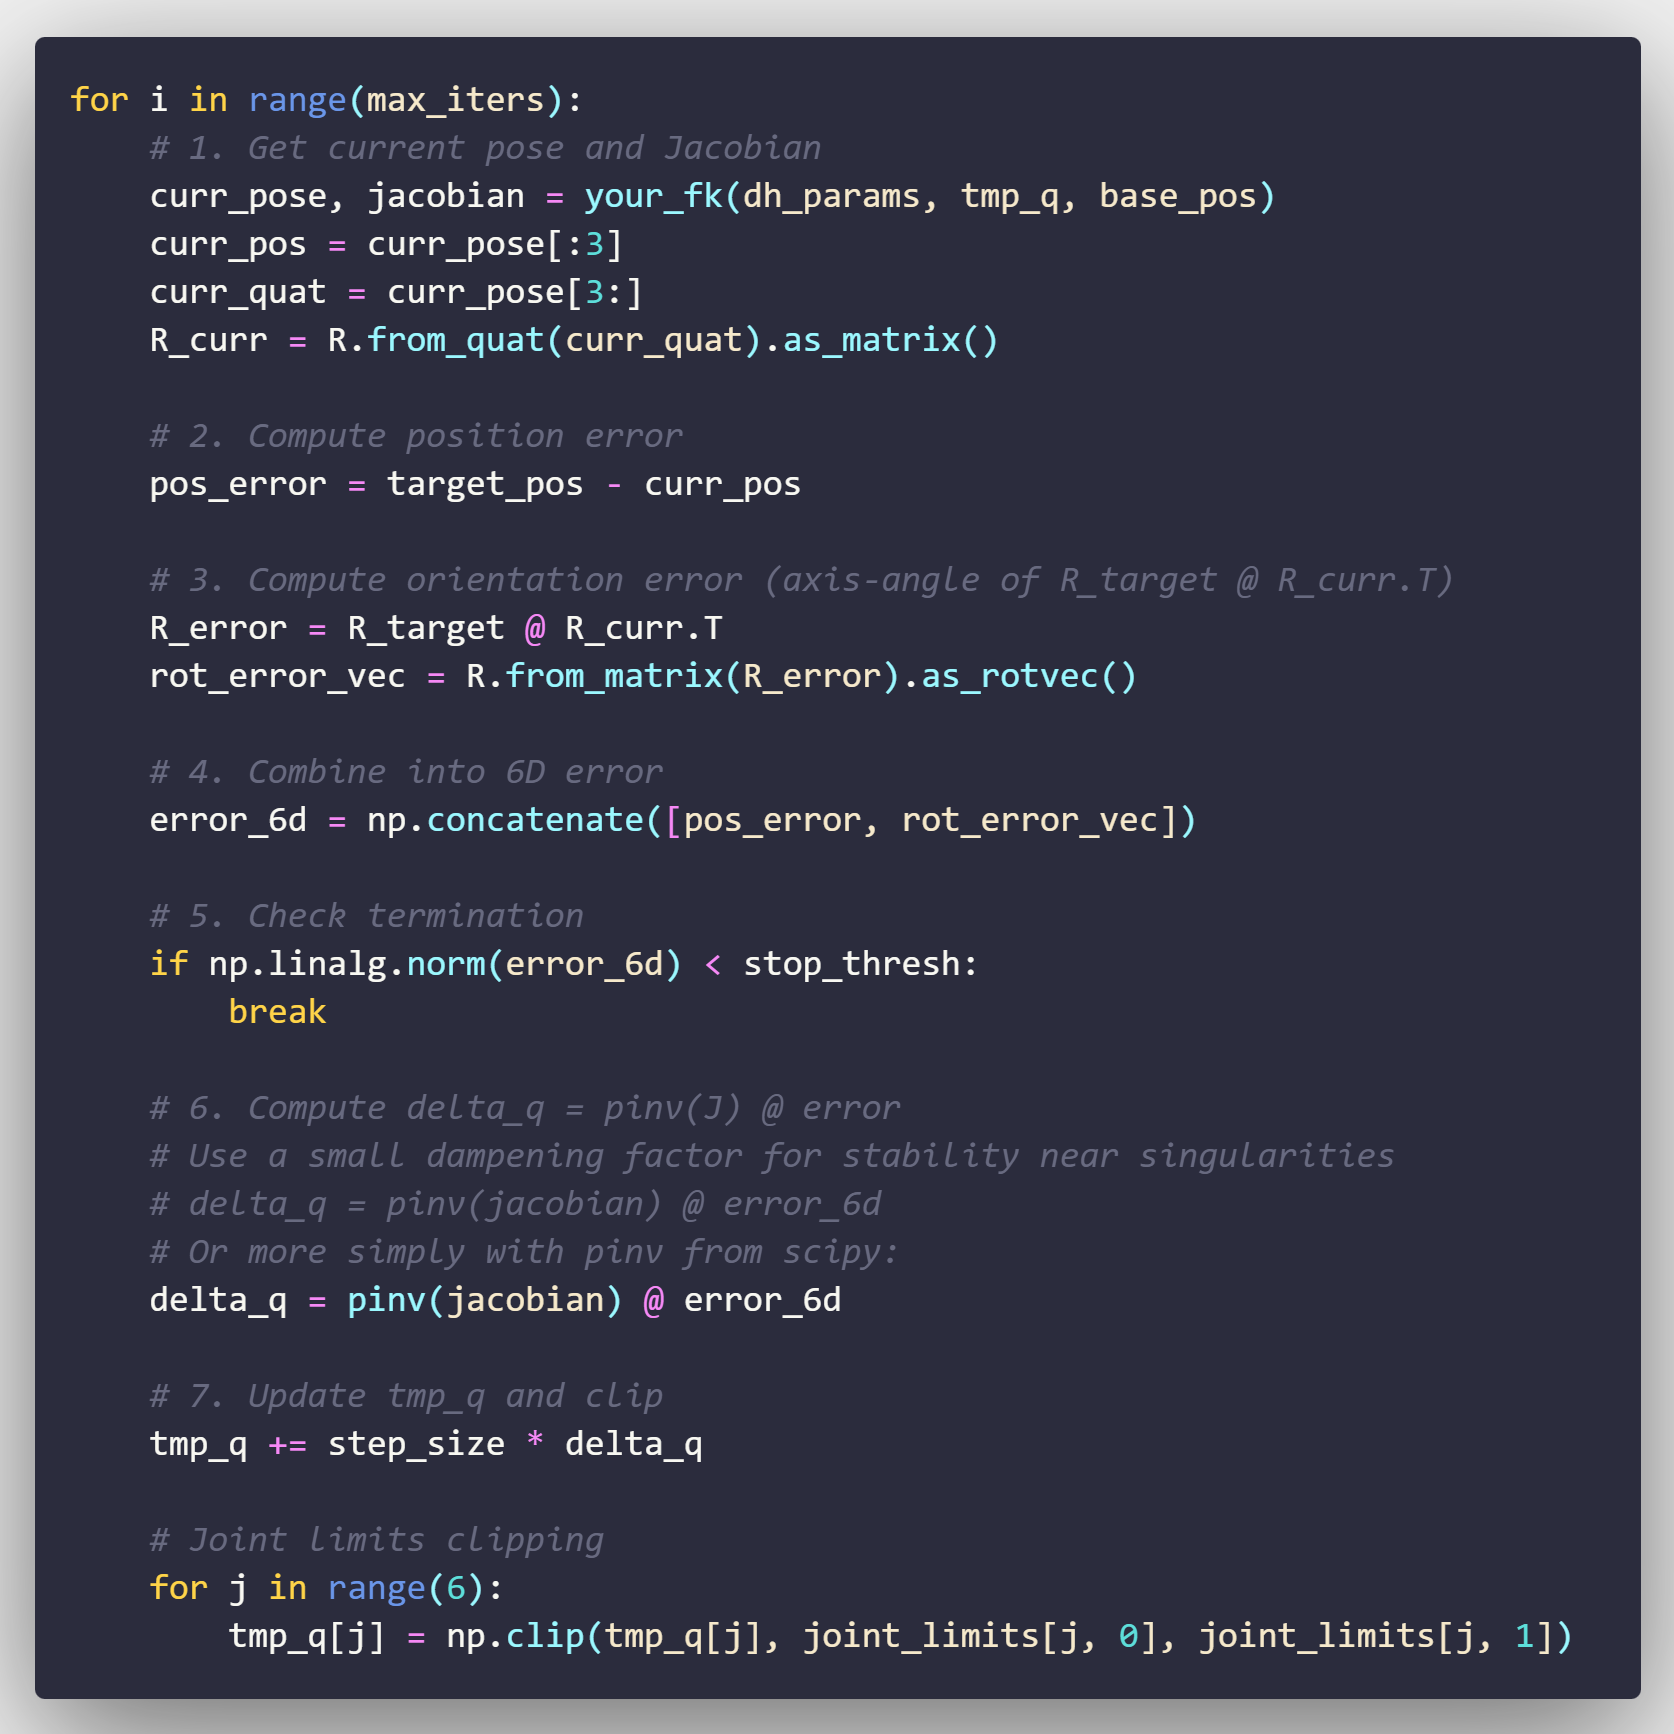
\includegraphics[width=0.8\textwidth]{screenshots/ikcode.png}
        \caption{Code snippet for the iterative IK solver using the Jacobian pseudo-inverse method.}
    \end{figure}
\end{enumerate}

\subsection{What problems do you encounter and how do you deal with them?}
The most significant problem encountered was that neither the headless nor the GUI tests for Task 1 and Task 2 could 
be executed on the glows.ai environment. The simulation would fail to initialize the graphics or physics engine, 
such that only a simulation window with empty content would pop up, and then fail with segmentation faults.

To resolve this, I modified the \texttt{SimulationApp} initialization logic in the scripts. 
Specifically, I explicitly configured the environment and GPU settings as follows:
\begin{itemize}
    \item \textbf{Environment Variables:} Manually set \texttt{CUDA\_VISIBLE\_DEVICES} and 
    \texttt{NVIDIA\_VISIBLE\_DEVICES} to ``0'' to force the application to recognize the GPU as a single-device.
    \item \textbf{Licensing:} Set \texttt{OMNI\_KIT\_ACCEPT\_EULA} and 
    \texttt{PRIVACY\_CONSENT} to ``Y'' to bypass interactive prompts in a CLI/Headless environment.
    \item \textbf{GPU Configuration:} Replaced the default \texttt{SimulationApp} 
    initialization with a detailed dictionary that explicitly assigned 
    \texttt{active\_gpu} and \texttt{physics\_gpu} to index 0 and disabled 
    \texttt{multi\_gpu} support.
\end{itemize}
This modification was essential for the simulator to successfully bypass hardware detection 
errors and carry out the kinematics calculations for the test cases.

\end{document}
